\chapter{Methods} \label{chapMethod}
\section{Datasets}
There is a lack of high-quality, organized, and consistent forestry data available for computer vision and robotics research. Therefore, a primary objective of this work was to collect high-quality datasets. In our early work, we focused primarily on collecting data from multiple sensors at once, so we could explore modern robotics approaches. In later work, we collected data from commodity drones that only capture geo-tagged images. This data is much easier to work with, but lacks the same richness as multi-sensor data.

\subsection{Commodity drone data}
Commodity drone data refers to data which can be acquired with only commercially-available tools and no specialized domain knowledge. In practice, a valuable and easy-to-collect source of data is GPS-tagged images collected in a pre-defined exhaustive survey. This can be obtained by even some of the smallest drones, such as DJI Mavic, which costs approximately \$1,600\footnote{\href{https://store.dji.com/product/dji-mavic-3-classic}{DJI Mavic}}. Commercial flight planners are a tool that allows a user to quickly define a survey region and fly over it in a geometric pattern. A common option is "lawnmower coverage" where a drone flies in a straight line, shifts over, and flies back the opposite direction. Another option is "grid coverage" where a lawnmower pattern is executed twice, in perpendicular directions. An important consideration when executing these surveys is the drone altitude, which represents a trade-off between coverage ability and spatial resolution. While drones can in theory fly to a substantial altitude, they are restricted in the US to 400ft and below due to concerns about interfering with crewed aircraft. The final consideration is front- and side-overlap. Front overlap refers to the fraction of the image which is observed in two consecutive frames captured as the drone is flying forward. The side overlap refers to how much overlap there is between neighboring flight lines.

In this work, we use several sources of commodity-level drone data. The first is actually collected with our more sophisticated drone. In these experiments, we only use the images from one camera and geotag them with our payload GPS. This is a reasonable analog for commodity drone data, since our camera and GPS are comprable to what would be found on a small commodity platform. 

The second source of data is taken from a study of structurally-complex western conifer forests \cite{Young2022}. This data was collected with a DJI Mavic in a lawnmower pattern at an altitude of 120 meters.

\subsection{Multi-Sensors Drone Data}
Many modern approaches to simultaneous localization (SLAM) and semantic mapping require as input multiple sensing modalities, such as cameras, LiDAR, IMU, and GPS. Therefore, other members of our team built a modular, multi-sensor payload that could be mounted on a drone. A render of the payload can be seen in Figure \ref{fig:methods:payload}. 

\begin{figure}
    \centering
    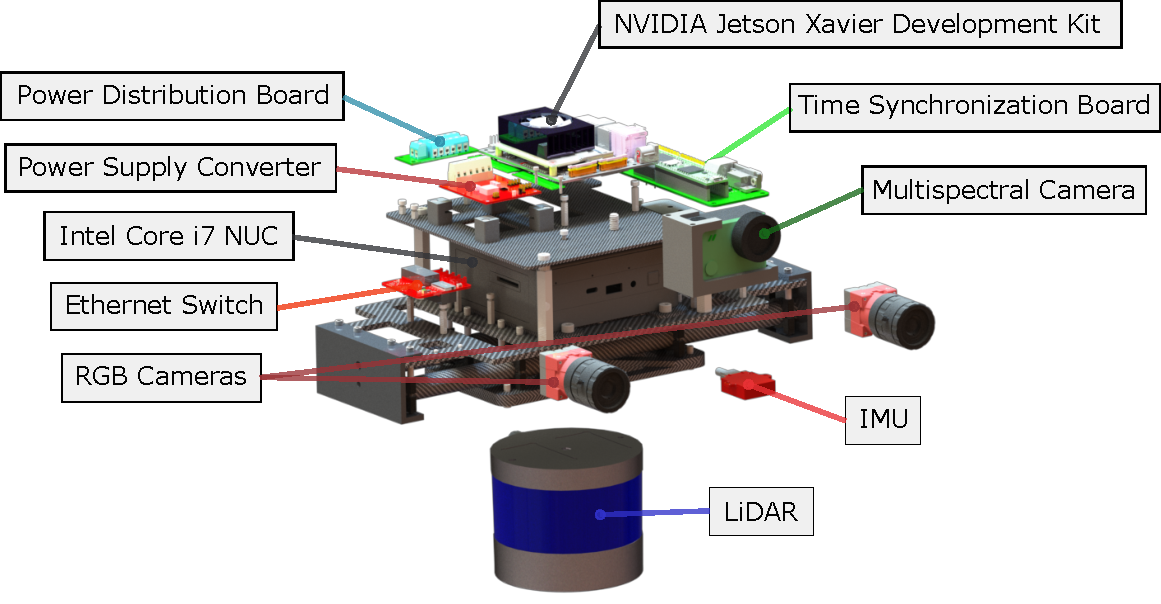
\includegraphics[width=0.55\textwidth]{figs/methods/datasets/payload_annotated.pdf}
    \hfill
    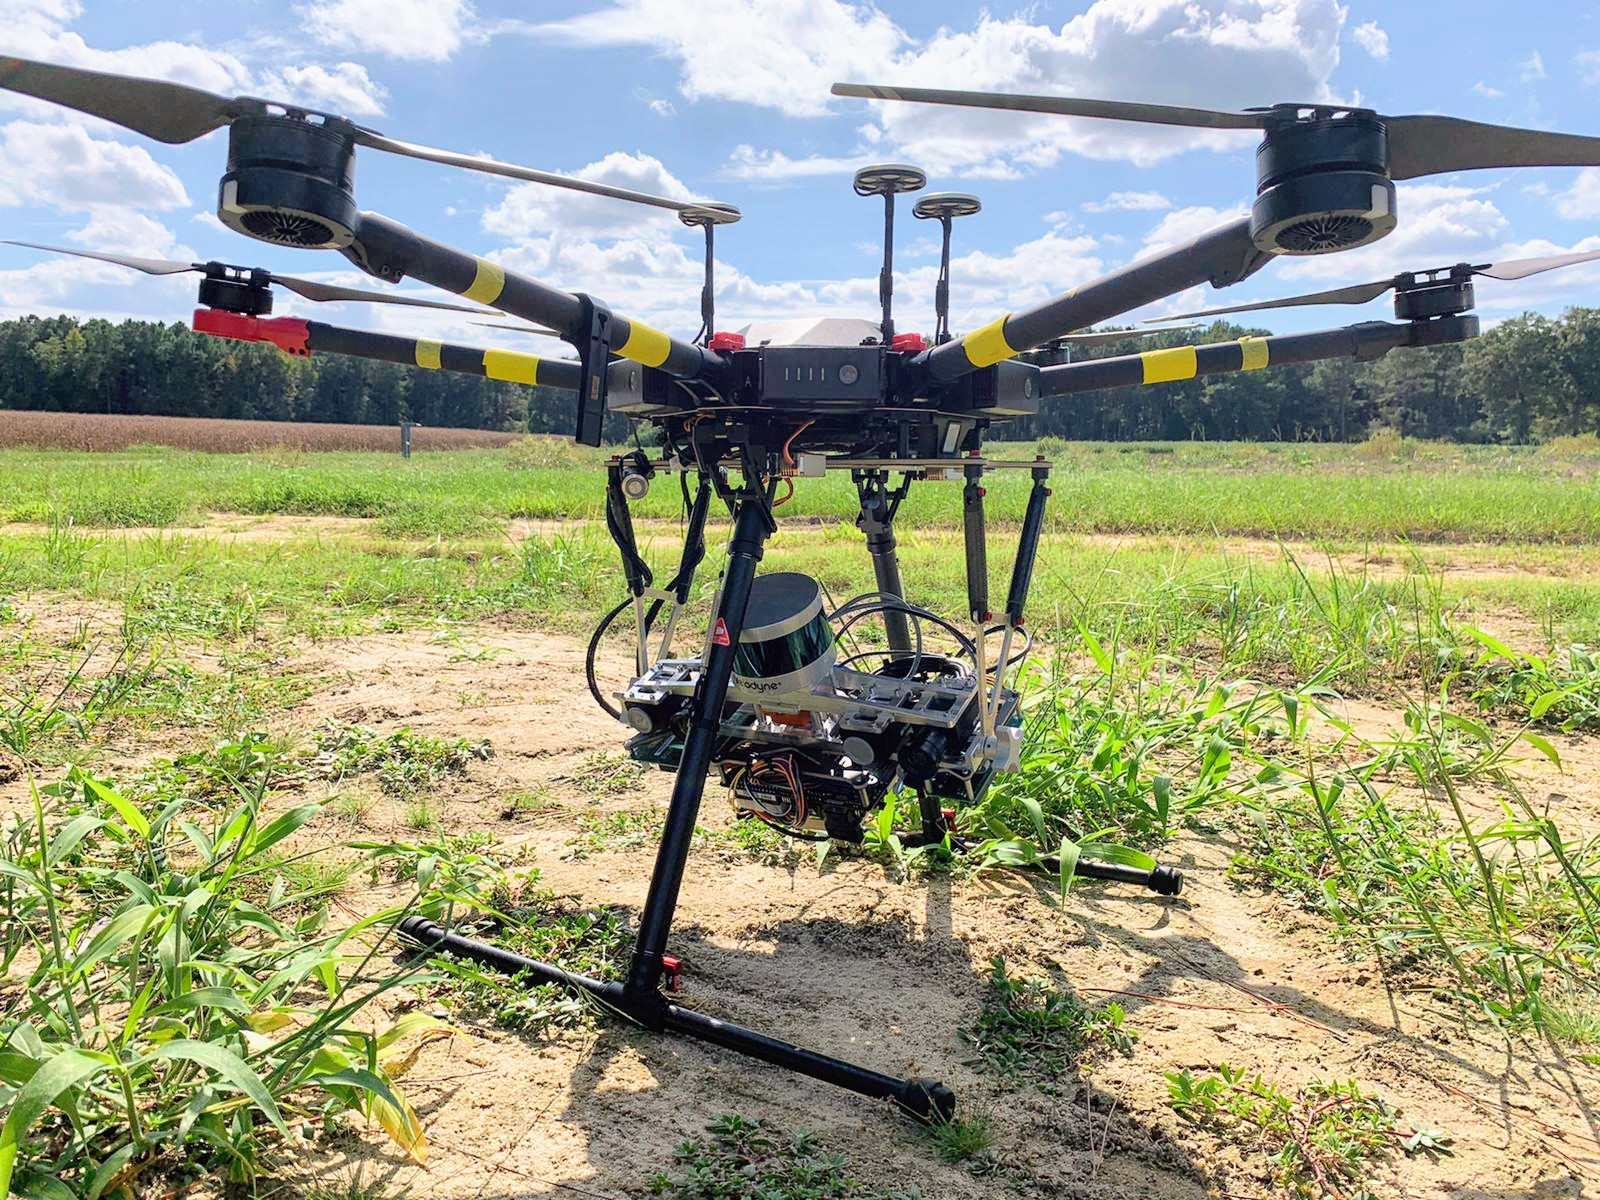
\includegraphics[width=0.37\textwidth]{figs/methods/datasets/payload_on_drone.jpeg}
    \caption{The multi-sensor payload designed by our collaborators. This was used for collecting rich forestry drone data. Photo credit to Winnie Kuang.}
    \label{fig:methods:payload}
\end{figure}

This payload is modular and could be mounted to different drones with different inclination angles. In these experiments, we used two large commercially-oriented drones, a DJI Matrice 600 and an AltaX Freefly. We flew a variety of different experiments, both under the canopy and over the canopy. In the under-canopy settings, we flew in small clearings between trees under manual control. Babak B. Chehreh from the University of Coimbra served as our pilot. In these experiments, we tried to survey the boundary of the clearing exhaustively by using an oblique payload orientation of 30 degrees from horizontal.

In the over canopy setting, we used a commercial flight planner. This allowed us to do a coverage plan over a region, using a traditional "lawnmower" pattern. Our altitude and overlap varied by experiment, but in most cases it was approximately 40 meters.


\begin{table}[]
\centering
\begin{tabular}{|l|l|l|l|l|}
\hline
\textbf{Name} & \textbf{Location} & \textbf{Platform} & \textbf{Environment} & \textbf{\makecell{Flight Pattern\\(camera degrees \\from horizontal)}}\\
\hline
Coimbra & \makecell{Coimbra,\\ Portugal} & \makecell{Multi-sensor \\ payload} & \makecell{Forest path} & \makecell{Manual out \\and back (30)} \\ 
\hline
Oporto & \makecell{Oporto,\\ Portugal} & \makecell{Multi-sensor \\payload} & \makecell{Forest clearing\\ with grass} & \makecell{Manual observations\\ of the boundary (30)}\\
\hline
Gascola & \makecell{Pittsburgh,\\ PA USA} & \makecell{Multi-sensor \\ payload}  & \makecell{Trees, shrubs,\\ and grasses} & \makecell{Lawnmower \\ over canopy\\ (75)} \\
\hline
Wharton & \makecell{Hammonton,\\ NJ USA} & \makecell{Multi-sensor \\ payload}  & \makecell{Forest with road} & \makecell{Manual oval \\ over canopy\\ (60)} \\
\hline
Stowe\{1,2\} & \makecell{Stowe,\\ VT USA} & \makecell{DJI Air 2s} & \makecell{Forest} & \makecell{Lawnmower (90)} \\ 
\hline
Emerald \cite{Young2022} & \makecell{Lake Tahoe,\\ CA USA} & \makecell{DJI Mavic 2} & \makecell{Forest} & \makecell{Lawnmower (90)} \\ 
\hline
\end{tabular}
\caption{A summary of drone datasets used in this work.}
\end{table}

\subsection{Non-drone Forestry Data}
We also used two existing sources of forestry data that were relavent to our domain. The first was a dataset of 121 images of a Portugese forest taken from a ground vehicle in the work of Andrada et. al. \cite{Andrada2020}. These images were manually labeled with six classes: Background, Live flammable material (aka Fuel), Canopies, Trunks, Humans, and Animal The original paper uses multi-spectral data but we just used the co-registred RGB data that was also releasted. This choice allowed us to deploy the model on a normal camera, rather than requiring a multi-spectral one. We refer to this dataset as \textit{Sete Fontes} because it was collected in a region with that name.

We also used a synthetic dataset rendered from a proceedurally-generated Portuguese forest \cite{nunes2021procedural}. In this work, the authors proceedurally-created a forested landscape by first creating the terain, the placing paths and rocks, and finally adding vegitation. Then they rendred images from this mesh. At the same time, they also a semantic image, that perfectly captured which class was observed at each pixel. These classes were slightly more-granular than those used in \cite{Andrada2020}, but they could easily be aggregated to match these. The exception was there were no examples of humnas or animals in this simulated dataset, but these were also rare in the Sete Fontes dataset and were not critical to this work. The synthetic dataset consisted of 3154 rendered images and associated sematic segmentation groundtruths taken at intervals from a simulated ground vehicle trajectory. 

\subsection{Optical remote sensing data}
In this work, we focus primarily on data collected by the National Aerial Imagery Program (NAIP) multi-spectral data source which contains red, blue, green and near-infrared bands. This data is collected at an interval of at most every three years over the continental US. The USDA contracts with states to obtain this data from manned aerial surveys. The data is post-processed to provide an ortho-rectified, stitched, and georefernced product analogous to satellite imagery. The resolution per pixel is 0.6 meters, which is relatively high for a free data product with a significant extent. An example image can be seen in Figure \ref{fig:methods:NAIP_example}.

\begin{figure}
    \centering
    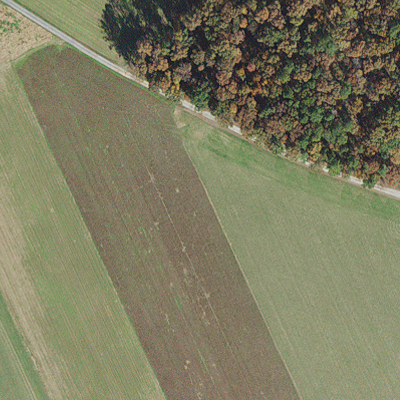
\includegraphics[width=0.5\textwidth]{figs/methods/datasets/NAIP_example.png}
    \caption{An example NAIP image crop.}
    \label{fig:methods:NAIP_example}
\end{figure}

\begin{table}[]
\centering
\begin{tabular}{|l|l|l|l|l|}
\hline
\textbf{Name} & \textbf{Location} & \textbf{Type} & \textbf{Environment} \\
\hline
Sete Fonte & \makecell{Coimbra,\\ Portugal} & \makecell{Under-canopy \\ images} & \makecell{Forest} \\ 
\hline
Synthetic \cite{nunes2021procedural} & \makecell{N/A, simulated} & \makecell{Under-canopy \\ images} & \makecell{Forest} \\ 
\hline
NAIP & \makecell{Continental US} & \makecell{Aerial imagery} & \makecell{Varied} \\ 
\hline
\end{tabular}
\caption{A summary of non-drone datasets used in this work}
\end{table}

\subsection{Data management}
A practical consideration when dealing with this much data is how to effectively store, version, organize, and share it in a seamless fashion, especially when working in collaborative teams. The tool used for managing the complexities of software development, such as `git`, have similar goals but do not support managing large, non-text files. 
Cloud hosting and local harddrives inenvitably become challenging to organize and do not natively support a versioning system, which makes them susceptible to accidental errors or duplicated data. 
In this work, we leveraged a software tool called Data Version Control (DVC), which is designed for organizing data in large projects such as machine learning and data science. DVC acts as a management layer between a git-tracked project and an arbitrary remote storage device. Effectively, DVC creates light plaintext files which describe the real data. These a small files can be tracked by `git` and represent a full history of the project.  

We created a `git` repo and associated `DVC` datastore for each project we worked on that had a different goal. Our organizational strategy evolved over time, but at the end involved two main concepts: a standardized hierarchy to organize the different data collects and a level designation to sort data based on the level of processing. The organizational structure was as follows `site\_name -> YYYY\_MM\_DD -> collect\_NNN` A site name represented one location where we collected data. This was chosen as the top-level organizational structure because data from the same site is most commonly used together. The next level represented the date and the final level broke the data up into logical segments. In general this corresponded to one drone flight, but in rare instances represented multiple flights where we left the sensors logging continuously, or data collected solely on the ground for calibration purposes. The level designation was inspired by the satellite community, where different levels denote different steps of sequential post-processing. In our work, we used Level0 to represent raw data, as copied from the platform. Level1 represented data processed into a standarized format. This was less important for commodity drone data, since it was frquently already captured as folders of geotagged images. However, it was very important for extracting easy-to-use information from rosbags, which is how our multi-sensor custom data was stored. Level2 represnted processed results such as structure from motion and semantic predictions. In initial work, we nested all the levels within a collect. However, we later found that for our usecases it was easier to have levels be the top level organizational structure. This allowed us to quickly check for all datasets matching a specific level of processing. The final organaiztional structure was as follows:

% TODO fix this up

\begin{verbatim}
    
├── level_00
│   ├── README.md
│   ├── <site_name_x> # A different folder for each geographic location
│   │   └── <date_YYYY_MM_DD> # A different folder for each day at that site
│   |       ├── collect_<NNN> # A different folder for each collect, which is probably synonmous with a flight
│   │       └── collect_<NNN>
│   └── <site_name_y>
│       └── 2023_06_15
│           ├── collect_<NNN>
│           └── collect_<NNN>
├── level_01 
│   ├── README.md
│   └── per_collect # Data in easy-to-use format, structured like level_00
│       └── README.md
└── level_02
    ├── README.md
    └── photogrametry # Photogramtery results
        ├── README.md
        └── metashape # Could have multiple softwares
            └── per_collect # Structured like level_00
\end{verbatim}

\section{Geometric understanding of forests using drone data}
\subsection{Photogrametry}
Data from commodity drones is very easy to use with structure from motion, since it is often provided as folder of images, with GPS information embedded in the EXIF metadata. This GPS information is not require, but provides a very helpful initialization to the structure from motion process. Furthermore, commodity drones are often set to only capture data at a low frequency or after traveling a given distance, to manage limited storage. Therefore, it is often advantageous to use all the available images. However, with our custom payload, the data was captured at a high frequncy of 10 HZ so consecutive images were often highly redundant. As shown by Young et. al. \cite{Young2022}, highly redundant images contribute little to the overall quality but we found them to dramatically increase computation times. Therefore, we the drone we downampled the image to 2HZ. If we had GPS data available, we tagged each image with the GPS coordinate from the temporally-nearest GPS record.   

After preliminary experiments, we found that a commercial software, Agisoft Metashape consistently produced high-quality results. We used the parameters found to work well by by Young et. al. \cite{Young2022}. In this study, the authors do not provide recommended parameters for the meshing step because this representation is not used in their pipeleine. Therefore, we used the default Metashape settings, which include "high" quality and "high" number of faces. In settings where we needed ortho-mosaics, or top-down renders, we also used the default settings. We conducted our experiments on high-end cloud infrastructure from the NSF Jetstream \cite{} program. 



\subsection{SLAM}    
Since SLAM is not the focus of this work, we choose to use results from our collaborators on these datasets. We use two methods from their experiments, LIO-SAM \cite{Shan2020LIO-SAM:Mapping} with the parameters tuned for the forestry domain and a custom SLAM that combines components of both LIO-SAM and VIL-SLAM \cite{Shao2019StereoMapping} to make an approach that combines information from both LiDAR and stereo vision in a tightly-coupled manner. A through description of this system can be found in \cite{RussellUnmannedMitigation}.


\section{Semantic Mapping of Forests}
The goal of our semantic mapping experiments was to determine what type of vegitation was where in the environment. We had a specific focus on accurately localizing fuel so that an automous ground robot could remove it. To accomplish this, we needed to both provide an accurate map of the world and add additional information to this map about what type of object was at each location.

Semantic mapping can be done with a variety of modalities. A relevant work on semantic mapping for forestry \cite{Chen2020SLOAM:Inventory}, focuses solely on detecting tree trunks within the environment. Because of the distinctive geometry of trunks, they are able to detect them in LiDAR. Because we want to distinguish classes that may have similar geometry, we choose to predict semantics using images, as done in the work of Andrada et. al. \cite{Andrada2020} in the ground vehicle setting. Using images has the added benefit that it is easy for humans to label annotated data to train the approach and to evaluate the quality of the predictions. Moreover, there is a wide range of semantic segmentation models available that are conceptually interchangeable. 

\subsection{Semantic Segmentation}
To the best of our knowledge, there are no pre-trained models that are useful for our task and publically available. Therefore, we needed to train our own models. We conducted two experiments, one on Portuguese data and another on the \textit{Gascola} we collected in the US. 

In the gascola experiemnts, our objective was to segment the different classes from overhead imagery. Since there weren't any relavent datasets, we chose to label a small ammount of data on our own for training. In semantic segmentation, it is very time consuming to label the boundaries between each class precisely. This is especially true for natural environments, where different classes are often interlaced at the boundary, such as tree branches over the ground or bare earth transitioning to grass. A relevant work on segmenting ground cover with drones is Davila et. al. \cite{Davila2022ADAPT:AI}, where they showed the coarsely labeling regions away from class boundaries was much faster and the model trained on these coarse annotaions still made good predictions at the boundaries. We conducted annotations using the VIAME toolkit, a free and open source web annotator pictured in Figure \ref{fig:methods:manual-annotations}. Even though our primary goal was to only distinguishes broad classes, we chose to annotate a more granular set of classes loosely inspired by the Anderson13 classes \cite{anderson1981aids}, a vegetation classification system commonly-used in fire modeling. Our reasoning was that this allowed us more flexibility when it came to future experiments, where we might want to aggregate the clsases differently. Furthemore, it gave us the option to train on these classes and aggreate them after prediction. In practice, we found that this additional granularity did not increase the labeling burden significantly, since we rarely had to break up spatial regions that would have originally been considered one coarse class. Rather, we mostly labeled entire regions with more granualar designations. 
To evaluate the performance of the model, we used another small annotated dataset from another flight over the same region. We summarized the IoU, precision, and recall for each class.

We use a segmentation network based on a transformer architecture called SegFormer \cite{Xie2021}. Given the relatively low amount of real-world images in our training dataset, this network was especially suitable since it showed strong performance on benchmark datasets and good generalization capabilities. We trained this model using the default parameters used in the MMSegmentation \cite{mmseg2020} implementation. 

Given the limited availability of real data and the labor-intensive nature of labeling to obtain ground truth, we explored the utility of models trained with simulated (\textit{synthetic}) data. We conducted three types of experiments: models trained solely with \textit{synthetic} data, models trained with real data (\textit{Setes Fontes}), and a mixture of both. For the last two cases, we trained with an increasing number of real images to evaluate the performance of the model with minimal real images. Thus, we conducted training experiments using (or adding) 7, 15, 21, 30, 60, 91, and 121 data points from the \textit{Setes Fontes} dataset. We trained for 10000 iterations and evaluated each model in 30 \textit{Setes Fontes} images not seen in the largest training split are used for evaluation and we replicate this experiment over five folds of the data. The three models are a fine-tuned implementation as the base networks were first trained with the \textit{CityScapes} dataset \cite{Cordts2016}.

\begin{figure}
    \centering
    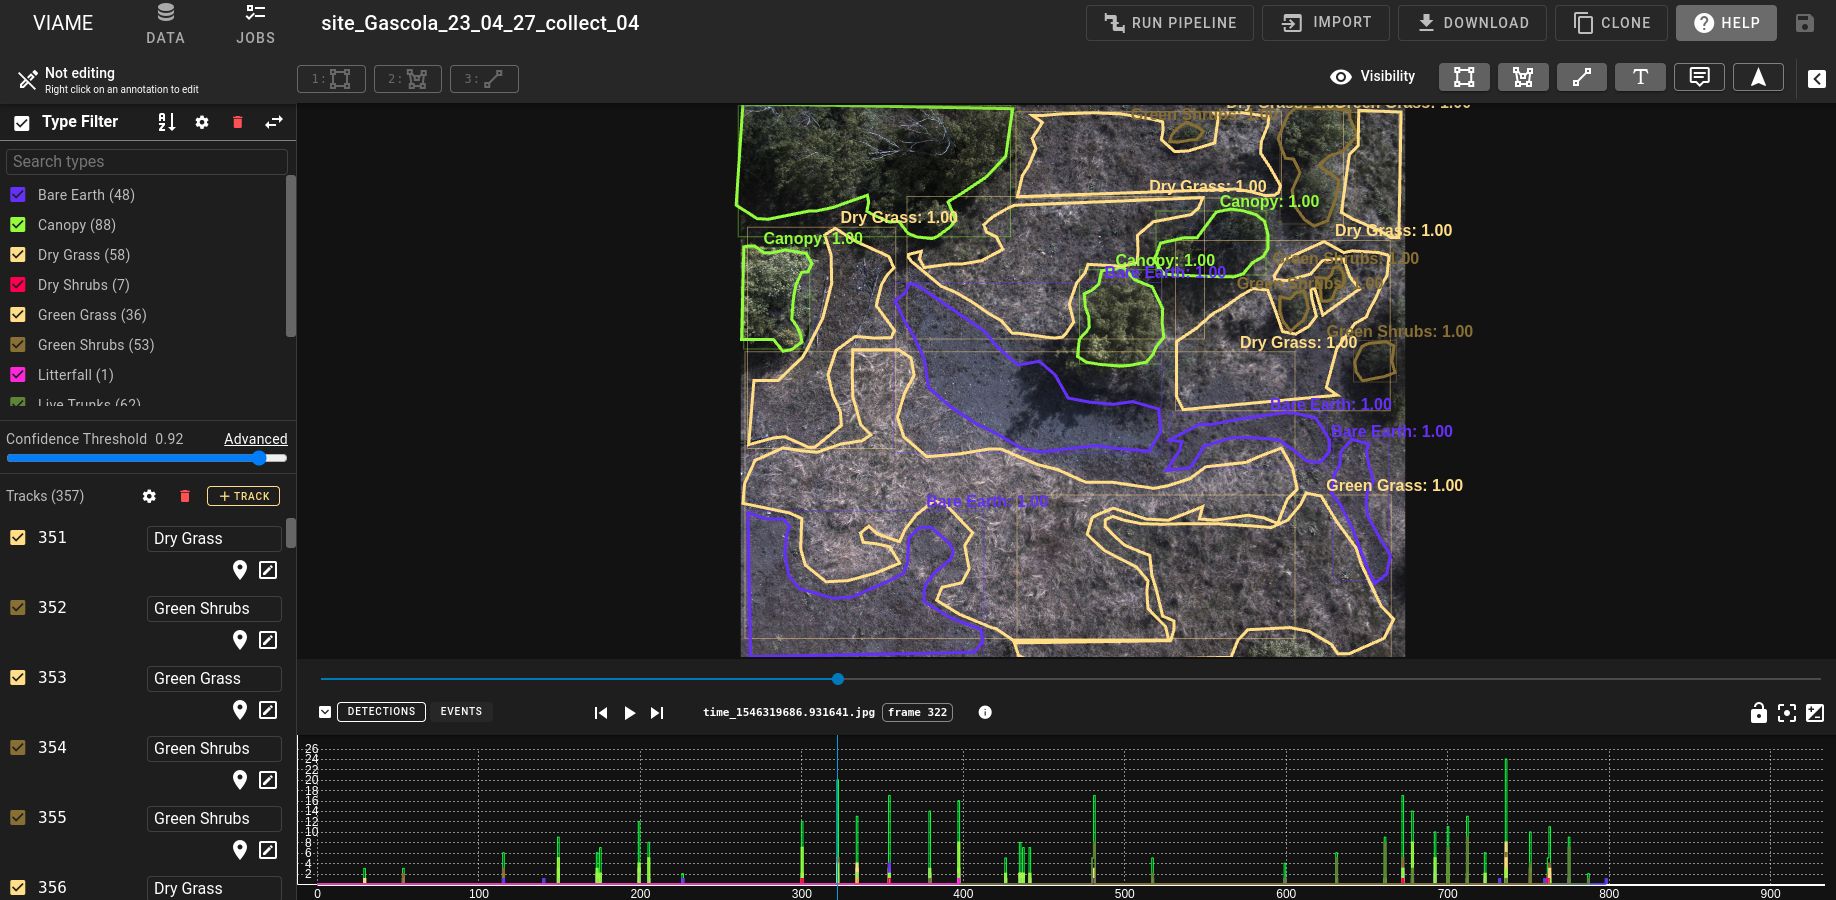
\includegraphics[width=\textwidth]{figs/methods/semantic_mapping/viame_example.png}
    \caption{Example manual annotations using the VIAME toolkit, a free and open source web annotator with potential support for integrated model training.}
    \label{fig:methods:manual-annotations}
\end{figure}

\subsection{Semantic Mapping with a Camera and LiDAR}

\begin{figure}
    \centering
    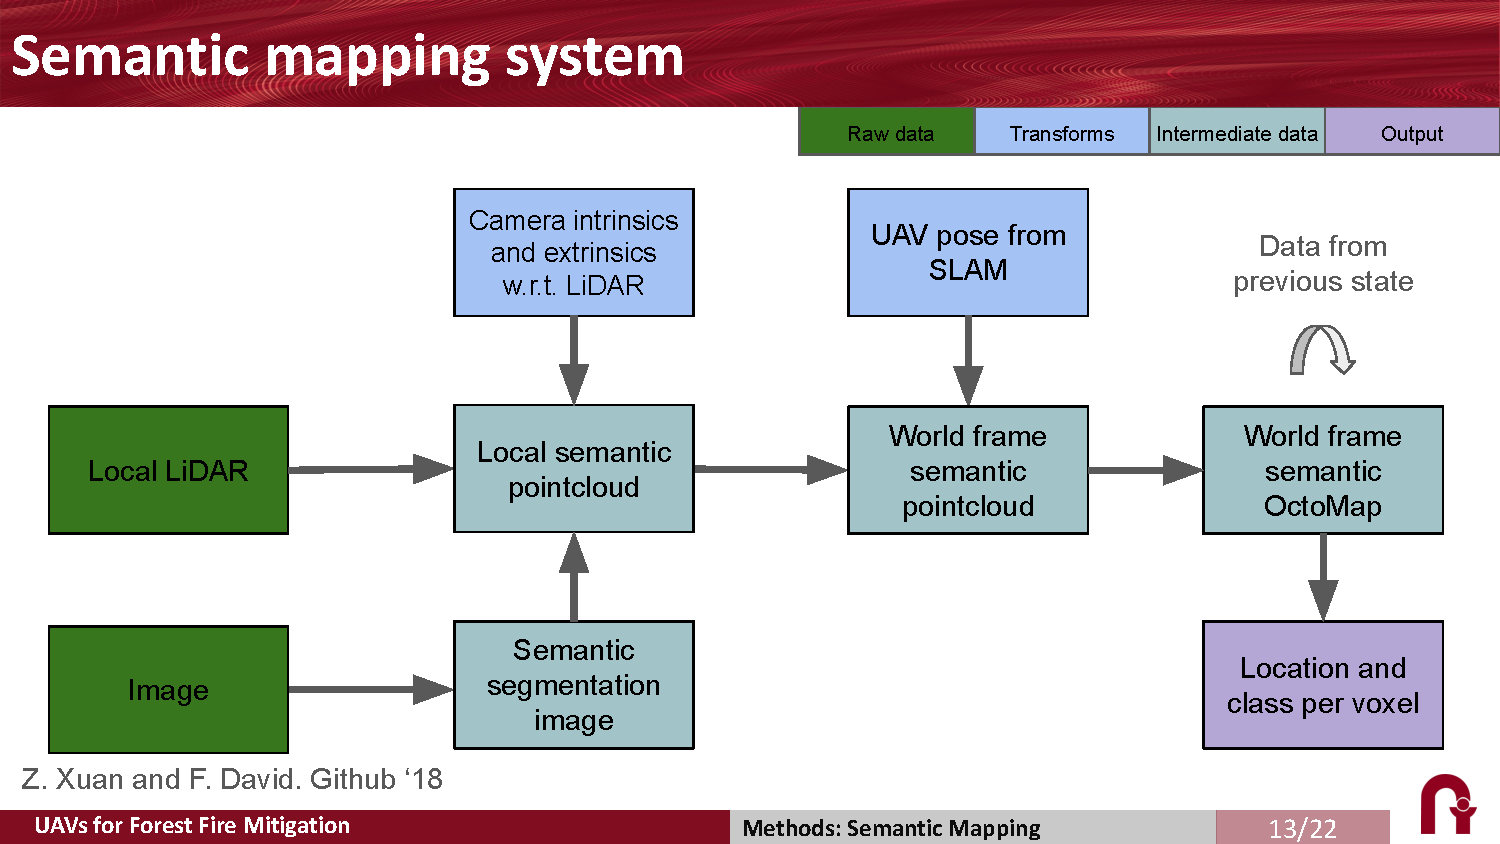
\includegraphics[width=\textwidth, clip, trim={0 1.5cm 0 1.8cm}]{figs/methods/semantic_mapping/semantic_mapping_overview.pdf}
    \caption{An overview of the LiDAR-camera semantic mapping system}
    \label{fig:lidar-camera-semantic-mapping}
\end{figure}

Subsequently, we modified an approach for RGB-D semantic SLAM \cite{semantic_slam} to project the detections from the image to the LiDAR domain (i.e., three-dimensional). First, the image is passed through the semantic segmentation network to get a classification result for each pixel. Using the extrinsics of the LiDAR relative to the camera, we transformed the LiDAR measurements into the camera's coordinate frame. Then, using the calibrated camera intrinsic, we project each LiDAR point into the image plane. Points within the field of view of the camera are assigned a classification label from the corresponding pixel in the semantic map. This semantically-textured point cloud is transformed into the inertial reference frame using the current pose of the drone estimated by our SLAM system. 

We use an octomap \cite{hornung13auro} representation to efficiently discretize the generated semantic point cloud into voxels. Each voxel has a resolution of 0.05m and contains information about the predicted classification. Each time a new semantic point cloud is created, it is used to update this global octomap. Since each voxel can contain multiple observations, we use two approaches to determine the aggregate classification. The first method assigns the class label using the highest-confidence prediction from the neural network that corresponds to that voxel. Alternatively, we use a Bayesian method which maintains a probability distribution over the classes. Each new observation is multiplied by the current distribution and then re-normalized. The voxel is then labeled with the most probable class.

%\subsection{Adding semantics to meshes}
%\begin{itemize}
%    \item The semantics are predicted for each image
%    \item The semantics are predicted onto the mesh faces
%    \item They are aggregated across the different viewpoints using...
%
%\begin{figure}
%    \centering
%    \includegraphics{example-image-a}
%    \caption{Single-view semantic prediction}
%    \label{fig:single-view-semantic-pred}
%\end{figure}
%
%\end{itemize}

\section{Tree detection in top-down data}
The goal of this work is to study tree detection at multiple scales, given a realistic set of operational constraints. Specifically, we assume that we have easy access to aerial or satellite data covering a broad region. This data is assumed to be at the lowest spatial resolution. Within this region, we have a drone survey which covers a smaller spatial extent but is at a higher resolution. Finally, we have an even smaller region where we know the location and extent of every tree. This could either be from field reference data or manual annotation of the drone data. An example of hte scale of the different types of data can be seen in Figure~\ref{fig:methods:multi_scale_tree_det}. Our goal is to accurately detect the trees in the entire region of interest that's covered by the satellite data. 

\begin{figure}
    \centering
    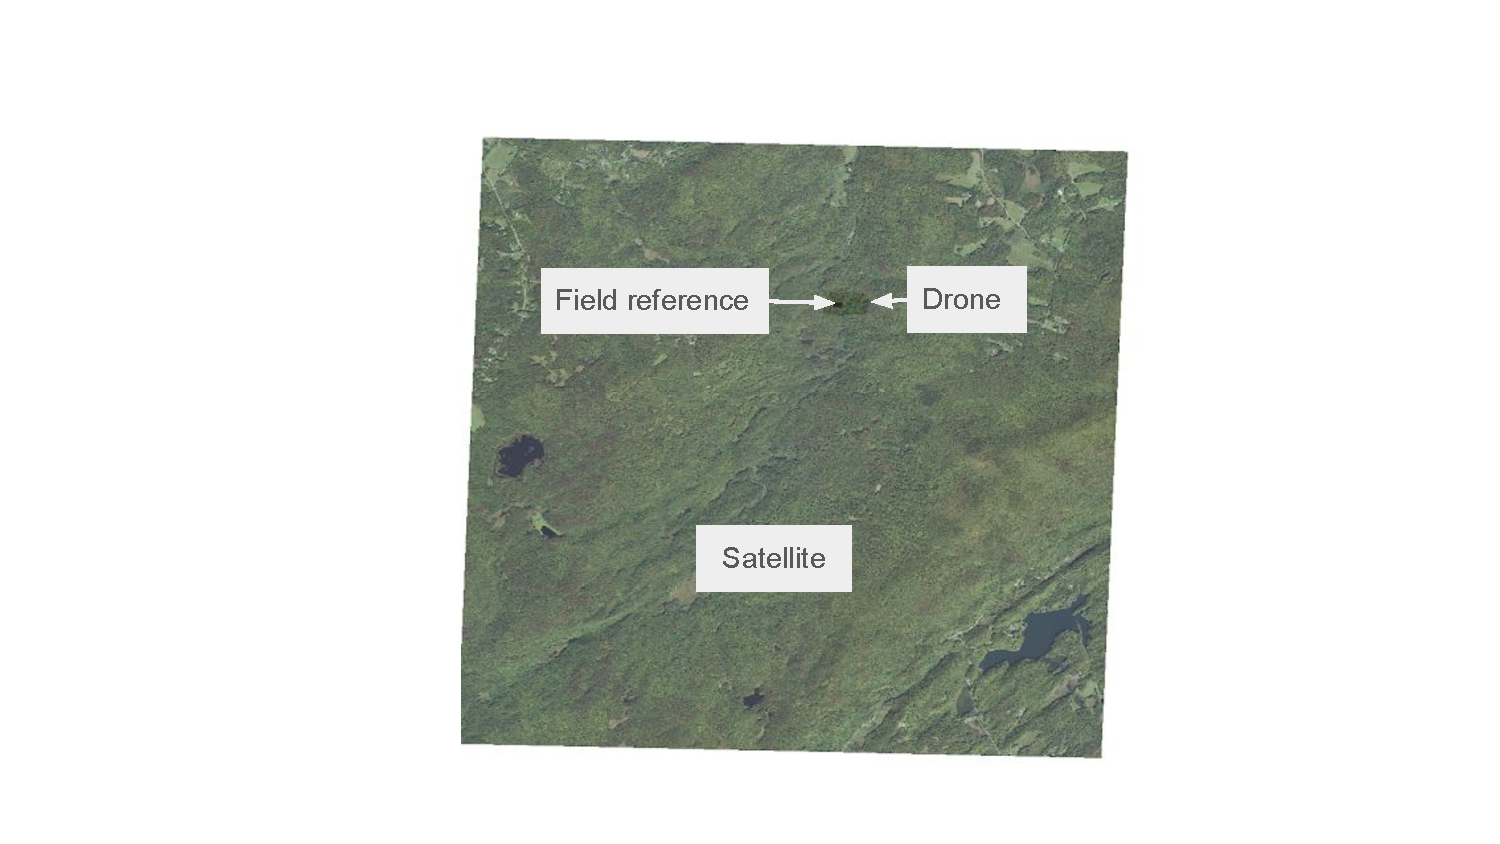
\includegraphics[width=0.7\textwidth, trim={6cm 0cm 5cm 1cm},clip]{figs/methods/tree_detection/multi_scale_data.pdf}
    \caption{Multiple scales of tree detection data}
    \label{fig:methods:multi_scale_tree_det}
\end{figure}
The first step in this experiment was processing the drone images into an orthomosaic, as described in the Photogrametry section. The orthomosiac was roughly geospatially regestered from the GPS readings where each image was taken. However, we noticed a translational error of several meters when the orthomosaic was overlaid on the NAIP data. Fixed translatinoal offsets are a common error with consumer GPS, though scale and rotation are often much more accurate. We fix this issue manually using an overlay in QGis to estimate the translational offset, and then updating the metadata using `gdalwarp`  

%We use a fairly common workflow which involves first building a 3D model of the scene, then rendering an orthomosaic, and finally generating predictions on the orthomosaic using a deep convolutional object detector. Specifically, we use the same Agisoft Metashape parameters as described in previous sections. We generate an orthomoasiac using the default settings, which leverages a mosaicing approach to generating the texture and blends the observations based on the mesh geometry. 



A widely-used method for tree detection in drone imagery is DeepForest \cite{Weinstein2020DeepForest:Delineation}, an object detection approach that was trained on a diverse set of semi-supervised tree annotations across the US. 


We then use DeepForest \cite{Weinstein2020DeepForest:Delineation}, which is a deep learning model trained on a diverse set of trees labeled in drone orthomosaics, to predict the bounding boxes for each tree in the image. An important consideration when using DeepForest is the geospatial input resolution, because this is known to have a strong impact on performance. Since our orthomoasics are in geospatial coordinates, we know the resolution in meters per pixel. Therefore, we resample the images to a consisent resolution of 0.1 meters per pixel, which matches the data that DeepForest was trained on.

To serve as training and test data, we manually labeled a small region of trees. 

\begin{figure}
    \subfloat{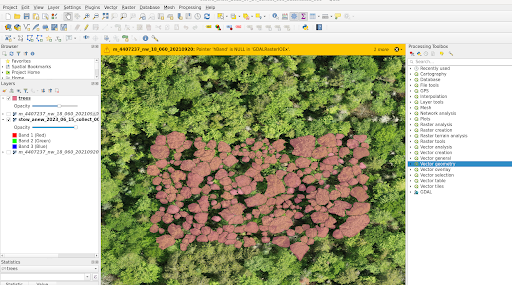
\includegraphics[width=0.45\textwidth, trim={4cm 0cm 3.5cm 2cm}, clip]{figs/methods/tree_detection/annotations.png}}
    \hfill
    \subfloat{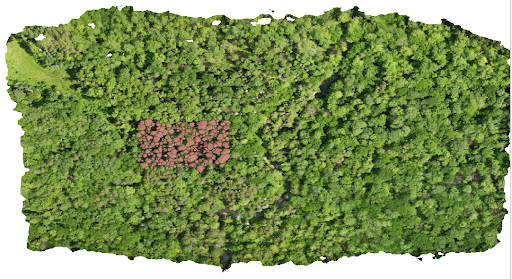
\includegraphics[width=0.45\textwidth]{figs/methods/tree_detection/annotations_scale.png}}
    \caption{Caption}
    \label{fig:enter-label}
\end{figure}

To conduct meaningful experiments with multiple types of geospatial data, it is important to have accurate registration. 

%The goal of this study is to understand the quality of tree predictions in satellite versus drone data. We also wanted to explore how much improvement a small set of annotations could yeild. Finally, we wanted to see how best to predict trees in a large expanse of satellite data using only a small number of labeled trees and a drone datasets collected around them.

\begin{itemize}
    \item TODO finish talking about the experimental setup 
\end{itemize}


\section{Informative path planning}

Since we have developed drone monitoring systems and shown how these observations can be extrapolated to a larger scale with satellite data, a natural question is where to collect observations with the drone. There are several factors we must take into account determining a sampling strategy. The first consideration is that drones have a finite battery life which governs the distance they can cover. Secondly, commodity drones require that their entire flight plan be specified before takeoff, and they do not provide functionality to implement re-planning strategies in flight. Thirdly, we make some simplifying assumptions to define the type of observations we take. Specifically, we assume that the atomic observation is a plot, or a small lawnmower survey of a fixed square size. We further assume that the user specifies a fixed number of plots to visit. Since it will take a fixed amount of time to execute the plot surveys, the maximum available time to traverse between plots is the maximum time of a full flight minus the time taken to complete the surveys. The algorithm's decision variables are where to place these plots and in what order to visit them, subject to the maximum time available to traverse between them.

In optimization problems, it is important to define a clear metric for desirable outcomes. The goal of our work is to collect samples that...
\begin{itemize}
    \item Talk about how we want these samples to be informative about the rest of the region 
\end{itemize}


\subsection{Feature extraction on remote sensing data}
\begin{figure}
    \centering
    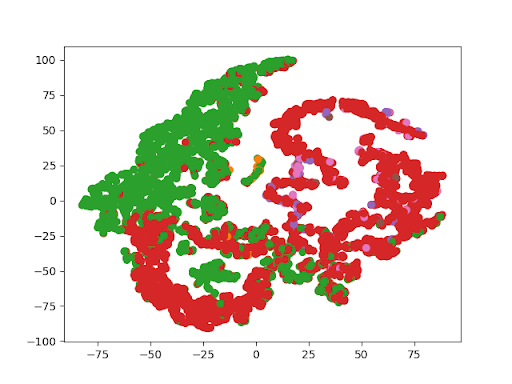
\includegraphics[width=0.5\textwidth]{figs/methods/IPP/TSNE_features.png}
    \caption{Unsupervised features seperate classes in a t-SNE embedding}
    \label{fig:methods:ipp_feature_embedding}
\end{figure}
We begin by running MOSIAKS \cite{Rolf2021}. Then we do dimensionality reduction with PCA or a VAE. This was motivated by the work of \cite{Candela2020PlanetaryMapping}. Then features are unitized. 

In this work, we need a system that can generate predictions from aerial/satellite data when trained on in-situ measurements such as species classification or biomass. Many domain-specific models exist for these tasks for a given modality. However, it is challenging to find or implement these models, especially for a non-technical domain expert. 

As we continued to work on this project, and guided by the report feedback, we realized the value of a prediction system that is explicitly designed to work with very few training samples. This is specifically helpful if we want to collect a single set of labels and then train a preliminary model to inform the next round of sampling. While there are many approaches from the field of low-shot learning, they are often complex and tailored to a specific task and domain. To reduce the complexity of our approach and try to develop a generalizable method, we leverage Gaussian Processes (GPs) \cite{Rasmussen2004} implemented in \texttt{GPytorch}\footnote{\url{https://gpytorch.ai/}}. This prediction system is common in many related works because it provides an explicit uncertainty, which can be used to inform sampling, along with the prediction. While GPs are often used for regression tasks, extensions exist for classification, such as \cite{milios2018dirichletbased}, which is implemented in \texttt{GPytorch}.

One major limitation of GPs is they are best suited to problems with several dozen features or fewer. Therefore, we must design a feature engineering strategy that produces useful features for these GPs to learn over. Directly using the channels of each satellite pixel does not capture the textures of the scene, which are important for moderately-high resolution data. While CNNs are commonly used for feature extraction, there is not the same diversity of pretrained models for satellite data as there are for other forms of imagery common in the computer vision community. However, recent work has shown than semi-random features are a strong alternative to even task-specific CNN features \cite{Rolf2021}. Specifically, this work proposes MOSAIKS, which are features computed by convolving random cropped patches of the image across the entire archive of satellite data. As shown in this work, these features are useful for a variety of downstream tasks. However, since the dimensionality of the feature vector is often in the hundreds or thousands (corresponding to the same number of randomly-sampled patches) it's too large to be used as an input to a GP. Therefore, we apply dimensionality reduction by using PCA to reduce the features down a reasonable number. In this case, we use 6. An example of this feature extraction method can be seen in Figure \ref{fig:unsupervised} and Figure \ref{fig:TSNE} shows that the features appear to separate nicely based on class.


    
\subsection{Gaussian Proccess uncertainty modeling}
\begin{itemize}
    \item Many works try to minimize the entropy of a Gaussian Proccess. This tool is especially nice because GPs can generate uncertainty predictions by only observing the features of a set of samples and not the labels.
\end{itemize}
\subsection{Remote-sensing Aware Planning Through Observation Randomized Sampling (RAPTORS)
}
\begin{figure}
    \centering
    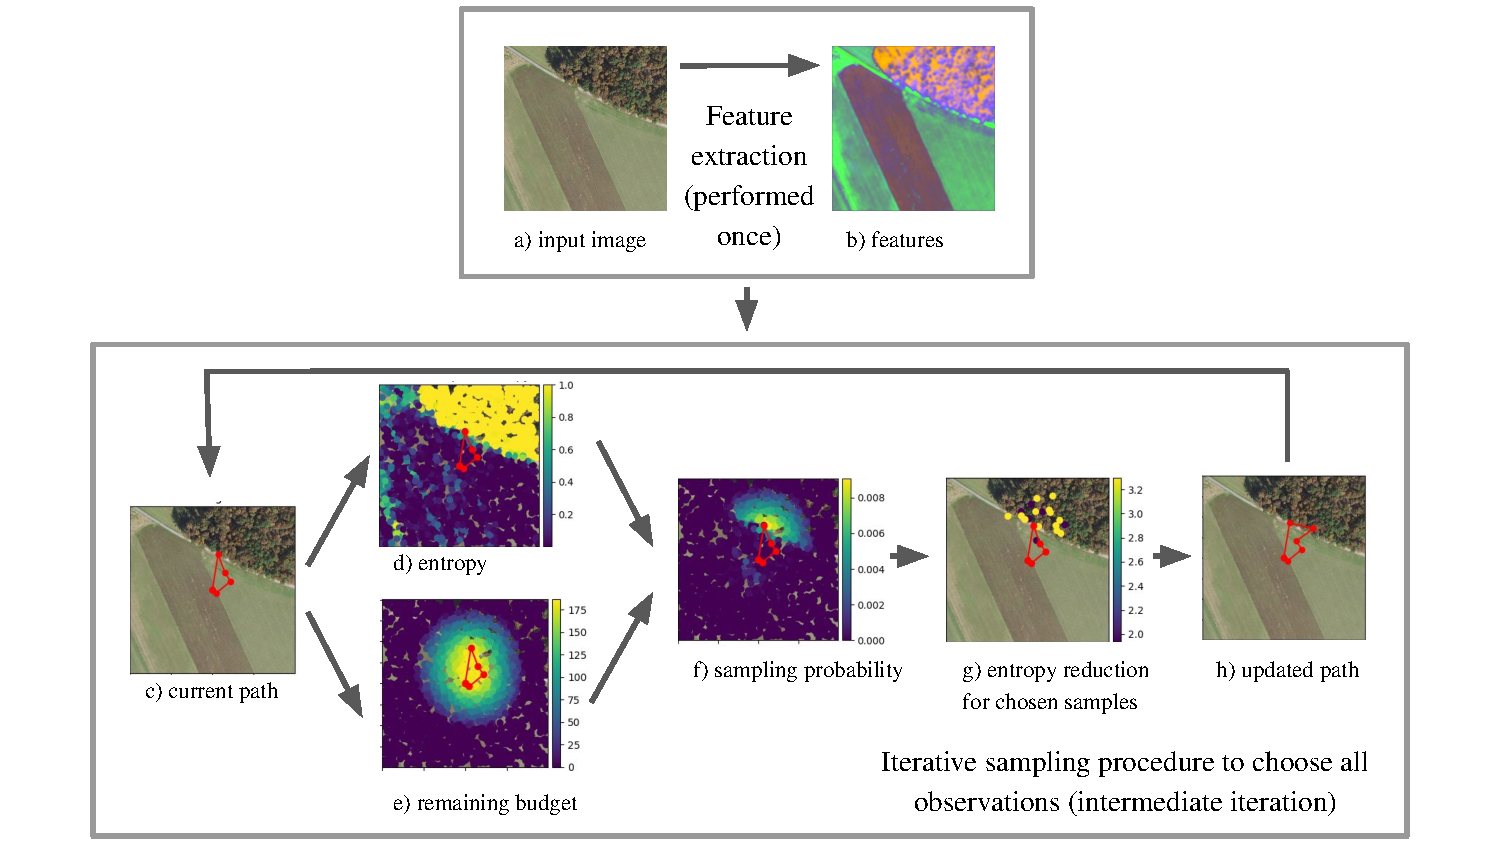
\includegraphics[width=\textwidth, clip, trim={1.5cm, 0, 1.5cm, 0}]{figs/methods/IPP/RAPTORS_concept_figure.pdf}
    \caption{This figure describes the workflow of a generalizable long-horizon path planner for selecting a set of drone observations. The required inputs are a satellite tile a), the drone's starting location, the path length budget, and the number of samples. Descriptive features are extracted from the image using random patches from the image as convolutional kernels, following the MOSAIKS method, and then compressed with PCA b). A full path is then built iteratively offline. At each iteration, the current path is provided as input, as shown in c). Then the uncertainty for a set of candidate locations is computed using a Gaussian Process d) and the remaining flight budget taking into account the current path is computed e). Then the uncertainty and remaining budget are multiplied and normalized to obtain a probability of evaluating each sample further. A set of samples are selected and the entropy reduction is calculated if each one were added to the Gaussian Process model f). Then the best sample is added and the path ordering is recomputed using a traveling salesman solver g). Then the process is repeated to plan the next observation until the requested number of observations are planned for. Only then is the path executed by the drone.
}
    \label{fig:methods:IPP_raptors_overview}
\end{figure}

\begin{algorithm}
\caption{RAPTORS}\label{alg:methods:RAPTORS}
\begin{algorithmic}
\State $F = extract\_features(I)$
\end{algorithmic}
\end{algorithm}

\begin{algorithm}
\caption{extract\_features}\label{alg:methods:extract_features}
\begin{algorithmic}
\State $F = extract\_features(I)$
\end{algorithmic}
\end{algorithm}

\begin{algorithm}
\caption{choose\_next\_sample}\label{alg:methods:choose_next_sample}
\begin{algorithmic}
\State $F = extract\_features(I)$
\end{algorithmic}
\end{algorithm}



 We employ a sampling-based strategy to build a long horizon offline path. This takes in an initial location, a number of samples, and a traversal budget. The algorithm begins by computing the gaussian process uncertainty after only observing the first location. Then, a feasible region is computed using a fraction of the remaining budget. A fixed number of samples are drawn from this feasible region, using a weighted sampling based on their uncertainty. The sample which reduces the total map unceratinty the most is added to the plan. Then the points are ordered using a TSP solver. The feasible region is recomputed using the added points and the fraction of the remaining budget.

\subsection{Problem formulation}
The goal of the experiments is to model a realistic data collection scenario. The data is collected over a series of missions, where each mission must be fully planned before it is executed. Each mission is allowed a pathlength budget and a number of samples it is allowed to collection. 

In our experiments we use randomly-sampled NAIP tiles to evaluate the approach. In each situation the agent starts in the center of the environment and must return there after each mission.

In these experiments we use a very simple prediction system to predict the class of unobserved pixels. It is simply a nearest-neighbor classifier which operates on the same PCA-compressed MOSAIKS features that are used for planning. While simple, this approach is well-suited to the extremely low number of training samples used in this setting and the standardized and uncorrelated nature of our feature space.

Before any missions have been executed, the agent can only observe the label of the pixel it is at. Then it plans a mission and executes it, observing the labels at the chosen sampling locations. These samples are used to train a prediction model which is used for evaluation and, in theory, could be used to inform the plan for the next mission. 


The experiments were conducted over ten random domains, which each represented an 800x800px crop from the Chesapeake Bay land cover dataset. Each tile represents approximately half a kilometer square. The pathlength was set as 800 pixels as well, which meant that the agent could go to one side of the environment and return to the start within the budget but some corners were completely unreachable. Each domain was explored using four missions where 10 samples could be collected during each one. Each sample meant the agent could observe the class of one pixel. After each mission, the class of all pixels  were predicted using the nearest neighbor classifier and the error metrics were computed. 


\subsection{Metrics}
The quality of the predictions are evaluated on two metrics, accuracy and averaged recall. The first is simply the fraction of pixels in the map that were assigned the correct class label by the prediction system. The second represents the average of the per class recalls. This metric is chosen so that rare classes are treated equally in the evaluation procedure, since this is critically important when we explicitly want to find rare classes. We also report the time taken to generate the plan. Note that this does not include the time taken to generate the class predictions, since the planner is agnostic to the choice of prediction algorithm.

 
 \begin{itemize}
     \item Talk about this in far more detail
     \item Add some more figures to describe the process
     \item Finish algorithm descriptions
 \end{itemize}